\chapter{Progettazione dell'architettura}\label{chap:architettura}
\section{Preambolo sulle scelte architetturali}
Le scelte archittetturali sono dipese in primo luogo dall'infrastruttura aziendale,
e successivamente dalle richieste avanzate negli incontri.
L'utilizzo di SQLServer, per il punti prima, è stato preso come base di tutte le scelte successive.
Da questo caposaldo si sono cercati dei framework che interagissero sia con SQLServer che,
 in ottica di offline, SQLite.\cite{SQLite}.
La scelta è ricaduta sull'architettura .NET\cite{DotNet} su base ``C\#'' che, in quanto dell'ecosistema Microsoft,
 è perfettamente integrata con i database.
Tale framework ha due pregi fondamentali per evitare i futuri debiti tecnici, ovvero:
\begin{itemize}
    \item supporta nativamente il multi piattaforma.
    \item ha una Community che lo aggiorna e supporta continuamente.
\end{itemize}
Selezionato questo package, si è scelto di proseguire con l'ambiente .NRT anche per la View.
La scelta è quindi ricaduta sul framework MAUI\cite{MAUI}.
MAUI è nativamente multipiattaforma in quanto, in fase di compilazione, genera i nativi sia per desktop che mobile.
I componenti della view sono anch'essi adattati alla piattaforma di esecuzione.
\section{Deployment}
La scelta degli ambienti di sviluppo prima citati, ha poratato alla creazione di un sistema che verrà 
installato ed eseguito in locale nelle singole workstation.
All'interno dell'azienda è presente un dominio \ac{AD} dove ogni Oggetto \ac{AD ha un }\ac{IP} statico,
La connessione al database, risiedente in un server all'interdo del dominio, avviene dunque mediante protocollo \ac{TCP}.
Si è valutato per chi accede dall'esterno del dominio di utilizza la \ac{VPN},
stabilendo una connessione virtuale come essere all'interno.
In assenza di connessione, verificabile tramite ping, si accede al database locale.
Una volta che si è ristabilita la connesione avviene la sincronizzazione con il database centrale.
\begin{figure}[h]
    \centering
    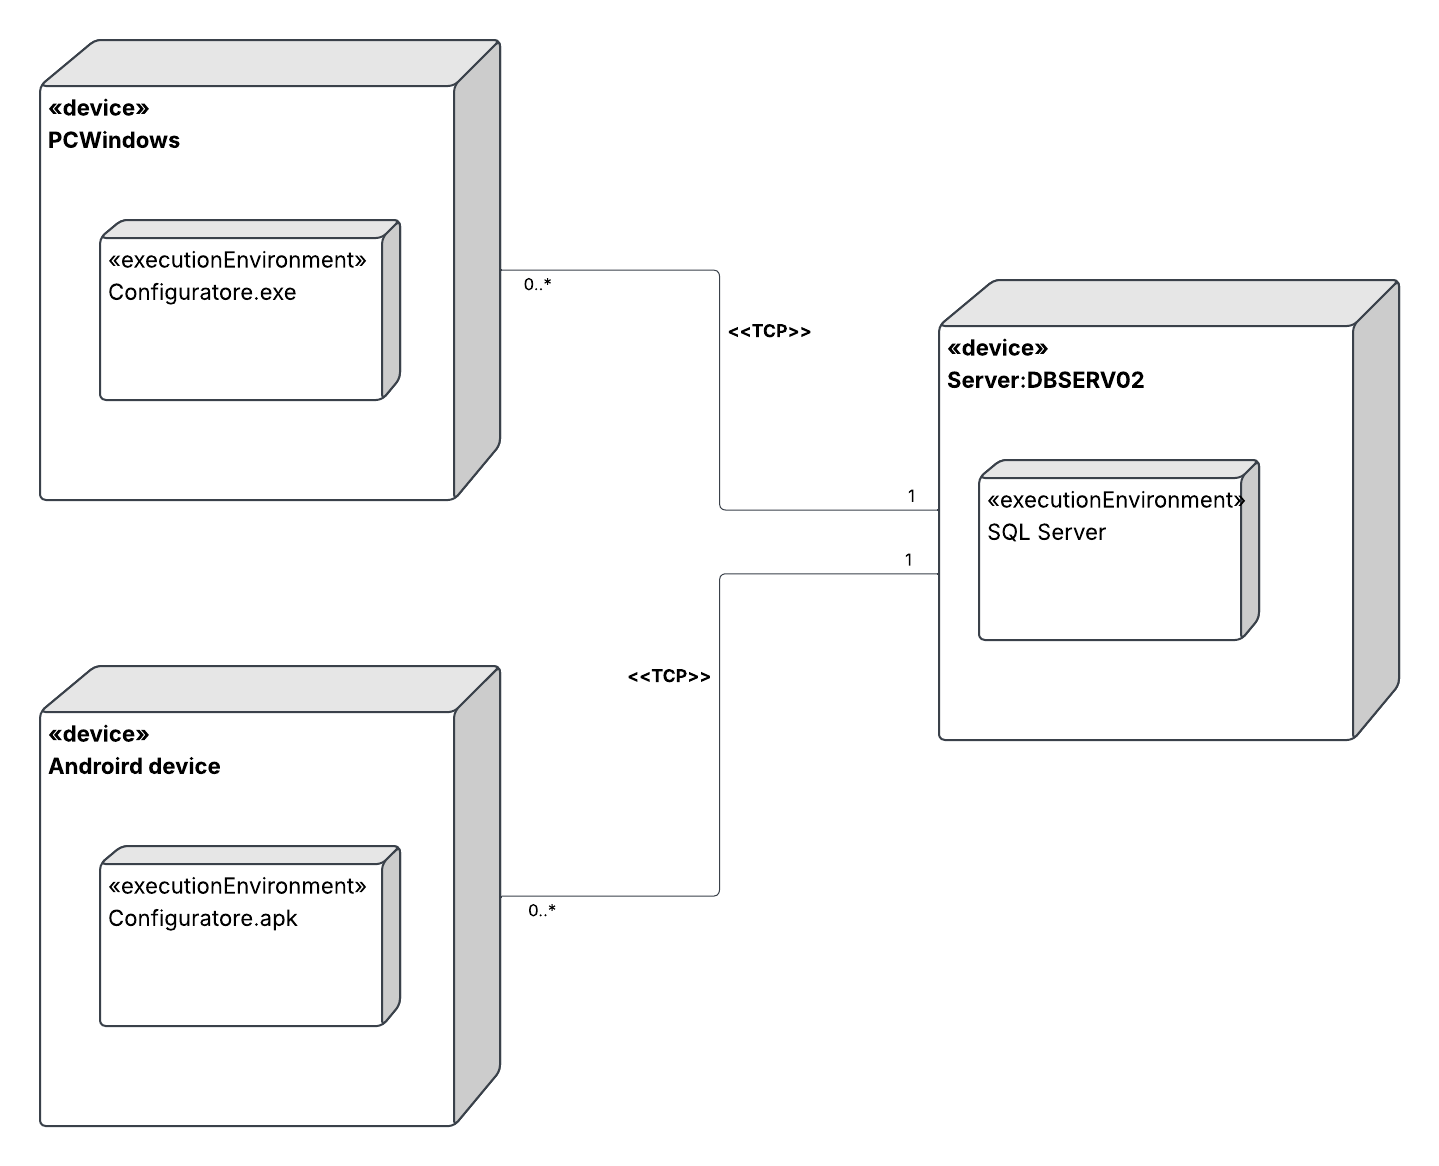
\includegraphics[width=1\linewidth]{figures/Deployment.png}
    \caption{Diagramma dei deployment}\label{fig:Diagramma dei Deployment}
\end{figure}
\section{Package}
La progettazione dell'applicativo ha portato a suddividerlo in tre Package con compiti ben distinti.
\subsection{Interfaccia al database}
Il package di interfaccia al database ha il compito di gestire tutti gli aspetti legati a quest'ultimo, come:
\begin{itemize}
    \item Gestire connesioni ai database.
    \item Gestione delle transazioni.
    \item Conversione, medinte \ac{ORM}, delle tabelle database in entity.
    \item Mappare entity in file neutri, proteggendo il database.
    \item Implementare tutte le operazioni ``CRUD''.
    \item Testare mediante classi di test le operazioni precedenti.
          Questa suite di test è risultata fondamentale per far fronte all'evoluzione del database nel corso dell'implementazione.
    \item Esporre al di fuori del package solo file neutri e classe di manager del database.
\end{itemize}
Questo modulo si appoggia a sua volta al pacchetto NuGet \ac{EF Core}\cite{MEF}, per quanto riguarda l'interazione col database,
ed il package ``Mapster''\cite{Mapster} per la mappature delle entity in \ac{DTO}.
\subsection{Libreria di componenti View}
Si è scelto di racchiudere le fatory degli elementi grafici, e delle costanti del dimensionamento delle stesse,
 in un package dedicato.
Il package è stato concepito a sé stante per favorire un suo impiego in altre applicazioni future.
La libreria si appoggia a sua volta al package NutGet ``Comunity Toolkit Maui''  dedicato al disegno dei compoenenti view MAUI.
Normalmente le interfacce MAUI sono scritte mediante codice XAML\cite{XAML},
 ma attraverso questo package si è potuto scriverle in ``C\#''.
\subsection{Modulo Main e View}
Il package principale ed il main del progetto è quello cge racchiude la gestione MAUI e di conseguenza delle interfacce grafiche.
Gli aspetti gestiti all'interno sono:
\begin{itemize}
    \item Creazione interfacce grafiche.
    \item Traduzione a compile time della conversione di codice "C\#" in XAML.
    \item Gestione delle interfacce mediante ViewModel , che a loro volta tramite observable modificano la view in risposta ad eventi.
    \item Gestione della navigazione tra le schermate.
    \item Gestione dei permessi, mostrando solo i comandi che competono al ruolo dell'utente.
    \item Mediante la classe MauiProgram.cs gestione della Dependency Injection.
    \item In fase di avvio creazione di una cache in RAM di dati immutabili durante la sessione, come tabelle di lookup.
\end{itemize}
\begin{figure}[h]
    \centering
    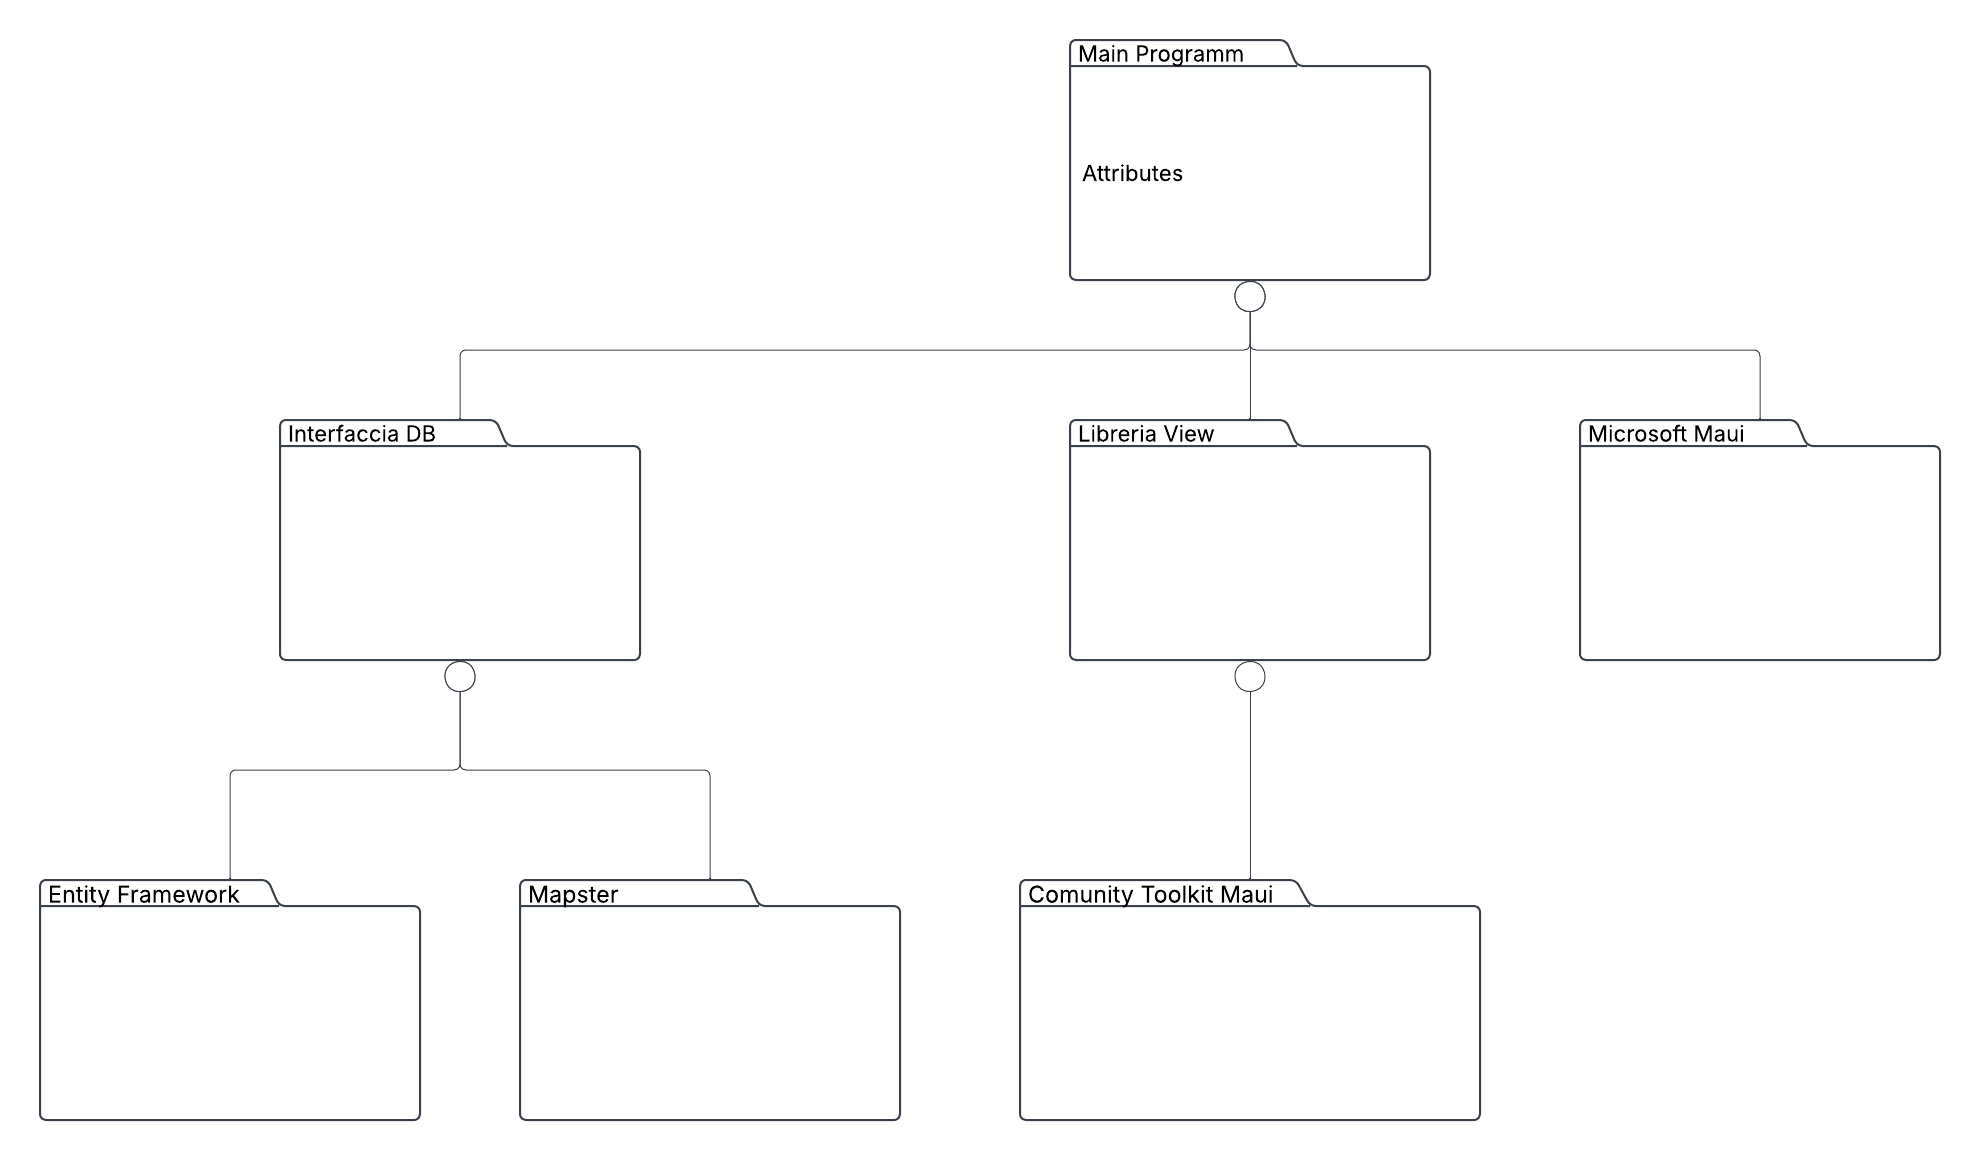
\includegraphics[width=1\linewidth]{figures/DiagramnaPackage.png}
    \caption{Diagramma dei package}\label{fig:Diagramma dei package}
\end{figure}
\section{Flussi di lavoro}
Osservando i requisiti si sono osservate delle problematiche relative all'attuale flusso aziendale del contratto.
Si è quindi studiato di inserire una revisione tecnica, da parte di un utente specializzato, del venduto.
Tale inserimento semplifica i flussi e facilita i reparti successivi.
Determinare tali flussi è fondamentale nel progettare gli automatismi a cui sono soggettele notifiche intra reparto.
\begin{figure}[h]
    \centering
    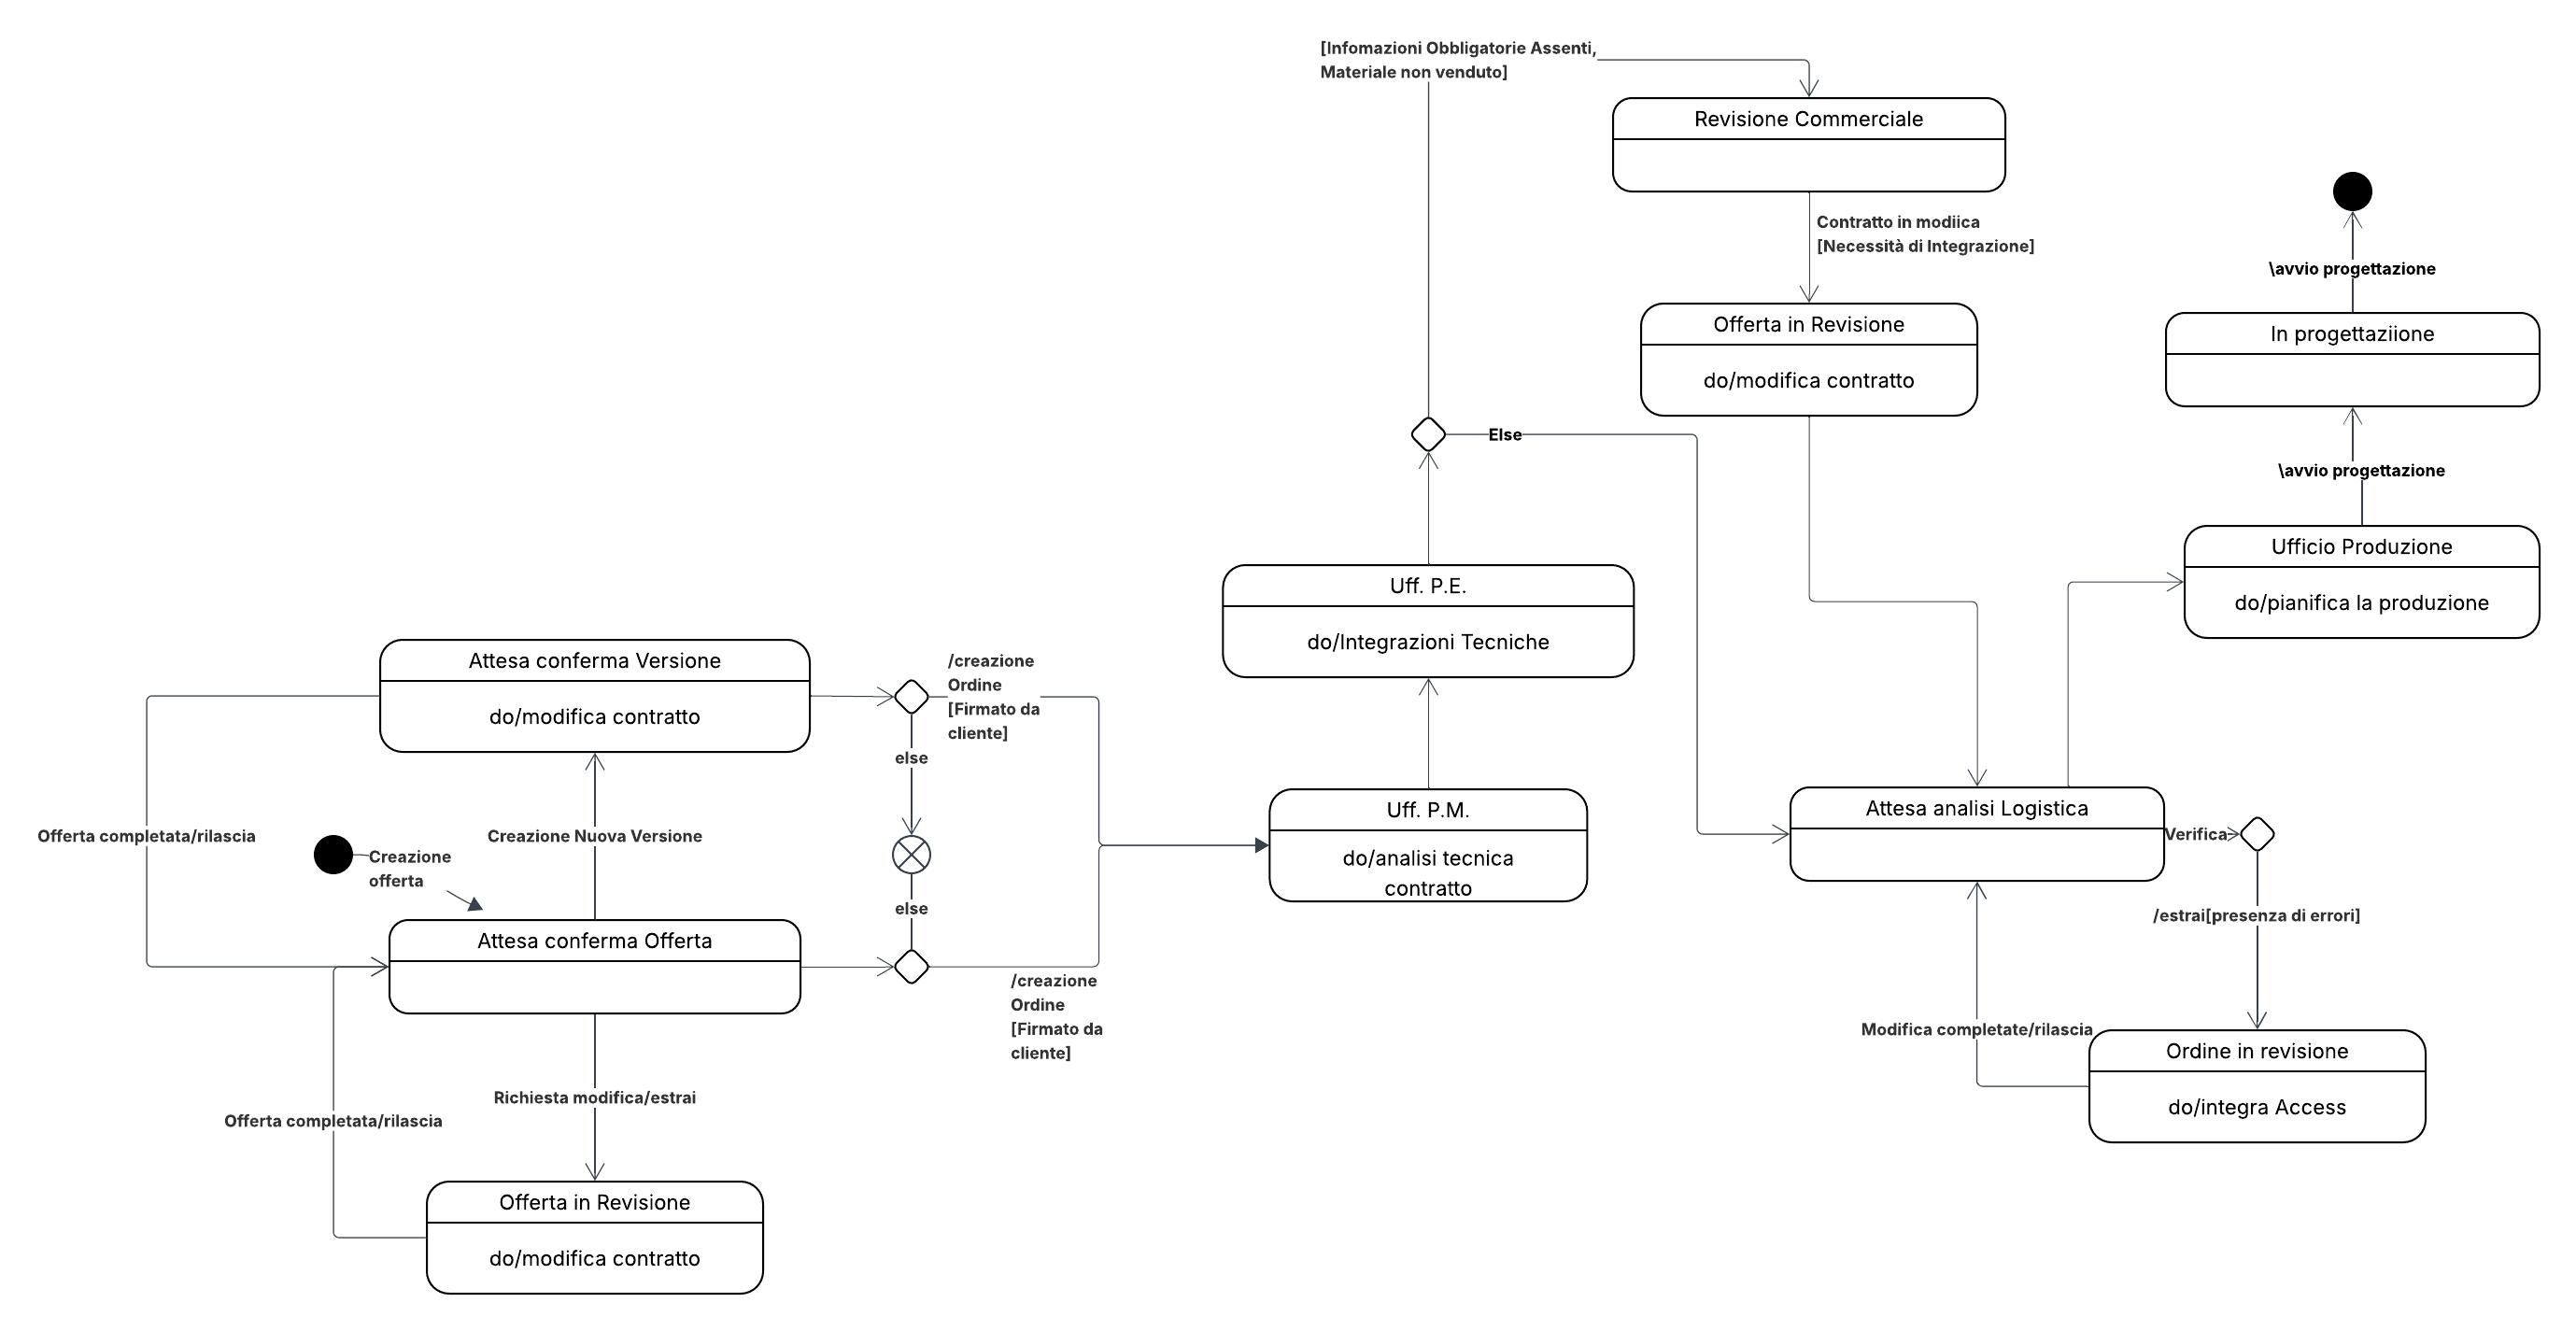
\includegraphics[width=1\linewidth]{figures/New Order flow.png}
    \caption{Nuovo diagramma degli stati di un contratto}\label{fig:Nuovo diagramma degli stati di un contratto.}
\end{figure}